\section{Results}

We have run our analysis over most of the SPEC CPU 2000 integer benchmarks, using the MinneSPEC reduced data input set \cite{KleinOsowski02minnespec}.
The results for our baseline model, along with the descriptions of the benchmarks as provided by SPEC \cite{henning00spec}, are provided in Table \ref{baseline}.
It can be seen from these results that none of these programs contain much task-level parallelism.
As we will see later, this is mostly due to the fact that the underlying algorithms of most benchmarks are necessarily sequential.
We will now proceed to describe the effects of different dependency models on our limits of parallelism, noting that while parallelism does not exceed single figures for any of the models we examine here, gains in relative terms will still give us insight on how greater parallelism may be found.
We will also suggest reasons why there is so little parallelism in these benchmarks, before providing some examples of other programs that exhibit much more parallelism.

\begin{table*}
\begin{tabular}{ | l | l | l | r | r | r | }
\hline
Benchmark & Language & Description & Serial length & Critical path length & Parallelism \\
\hline
164.gzip & C & Compression & 852994275 & 836250530 & 1.020 \\
175.vpr\_place & C & FPGA Circuit Placement & 30015847 & 28888197 & 1.039 \\
175.vpr\_route & C & FPGA Circuit Routing & 9008077 & 6688489 & 1.347 \\
176.gcc & C & C Programming Language Compiler & 102875883 & 83960956 & 1.225 \\
181.mcf & C & Combinatorial Optimization & 160615720 & 74266623 & 2.163 \\
186.crafty & C & Game Playing: Chess & 166315214 & 153019717 & 1.087 \\
197.parser & C & Word Processing & 391853645 & 361559175 & 1.084 \\
252.eon\_cook & C++ & Computer Visualization & 396417460 & 178717581 & 2.218 \\
252.eon\_kajiya & C++ & Computer Visualization & 528195627 & 251127042 & 2.103 \\
252.eon\_rushmeier & C++ & Computer Visualization & 383335201 & 168056567 & 2.281 \\
253.perlbmk & C & PERL Programming Language & 194675347 & 192775902 & 1.010 \\
254.gap & C & Group Theory, Interpreter & 80099675 & 75660828 & 1.059 \\
255.vortex & C & Object-oriented Database & 97266720 & 80887698 & 1.202 \\
300.twolf & C & Place and Route Simulator & 129292883 & 117049408 & 1.105 \\
\hline
\end{tabular}
\caption{Description of and baseline figures for the SPEC CPU 2000 integer benchmarks}
\label{baseline}
\end{table*}

\subsection{Data dependencies}

\begin{figure}
 \centering
 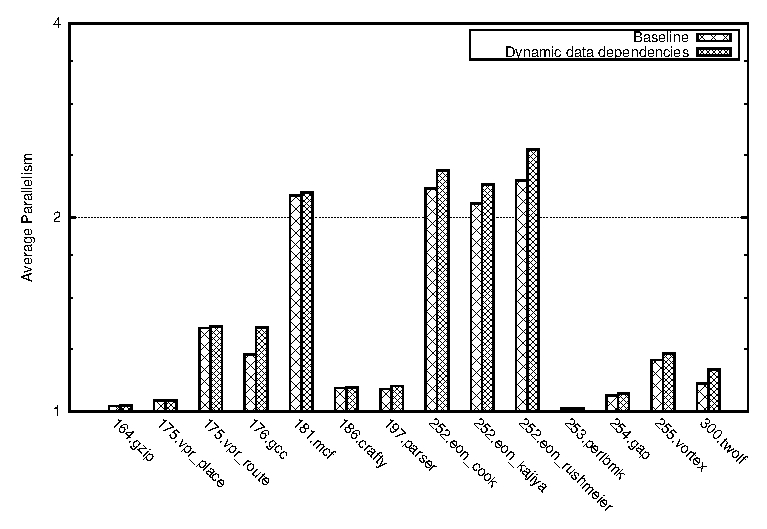
\includegraphics[width=3in]{spec-data}
 \caption{Limits of parallelism with static and dynamic data dependencies}
 \label{spec-data}
\end{figure}

Figure \ref{spec-data} shows the parallelism limits when considering dynamic data dependencies compared to the baseline model of using static dependencies.
It is perhaps surprising to note that for many benchmarks the use of dynamic dependencies does not give much of an advantage over static dependencies (in fact it gives only a 3.3\% speed-up on average over the baseline), suggesting that dependencies are perhaps fairly consistent over the execution of a program.

\subsection{Control dependencies}

\begin{figure}
 \centering
 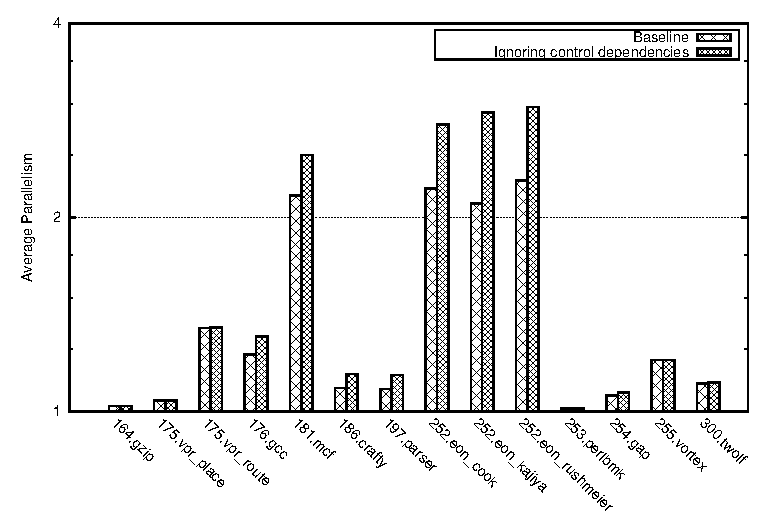
\includegraphics[width=3in]{spec-ctl}
 \caption{Limits of parallelism with and without static control dependencies}
 \label{spec-ctl}
\end{figure}

Figure \ref{spec-ctl} compares the limits of parallelism when ignoring control dependencies to those of the baseline.
Ignoring control dependencies models the effects of perfect control speculation.
Here we see that a few benchmarks show a significant improvement, at least in relative terms, when control dependencies are ignored.
The speed-up of Eon ranges between 25\% to 40\%, and the average speed-up across all programs is 9.2\%.
These figures suggest that control speculation is a valuable technique for increasing parallel performance.
As noted, simple branch prediction (e.g.\ predicting the same branch as the one last taken) is sufficient for high accuracy \cite{smith98study}, and consequently we believe that such improvements should be attainable.

\subsection{Line-level parallelism}

\begin{figure}
 \centering
 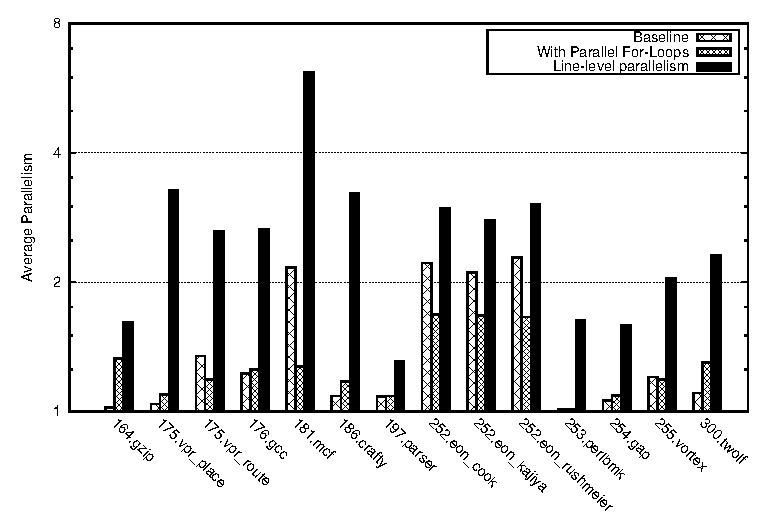
\includegraphics[width=3in]{spec-gran}
 \caption{Limits of parallelism of different granularities}
 \label{spec-gran}
\end{figure}

The rightmost columns in Figure \ref{spec-gran} shows the improvement in parallelism when considering line-level parallelism, which averages 91\%.
Some benchmarks which thus far have displayed hardly any parallelism begin to exhibit more, although it is still low in absolute terms.
It is unknown how much of this line-level parallelism is too fine-grained to be exploited by multi-processors.
Nonetheless, the results suggest that perhaps we should look closer at other ways of delineating tasks, in addition to using function calls, in order to achieve greater parallelism.
This model also does not in general include loop-level parallelism, as we cannot distinguish between loop-independent and loop-carried dependencies in our current static model, meaning that parallel loops would still be linearised.

\subsection{Loops}

The middle columns in Figure \ref{spec-gran} show the limits of parallelism when natural loop iterations are also spawned as tasks in the same way as function calls.
They show the effects of exploiting DOALL parallelism, where loop iterations that are completely independent from each other can be executed in parallel.
At the same time, however, spawning a task for each loop iteration means that if there are cross-iteration dependencies then no parallelism is possible, thus precluding DOACROSS parallelism or software pipelining.
The balance between DOALL and DOACROSS loops would therefore determine whether parallelism rises or falls compared to the baseline.
The results, as expected, show a mixed picture.
Benchmarks such as gzip and twolf show a marked improvement, as they appear to have a few DOALL loops.
Others, such as mcf and eon, show an even bigger degradation, due to the presence of DOACROSS parallelism.

\subsection{Spawn hoisting}

\begin{figure}
 \centering
 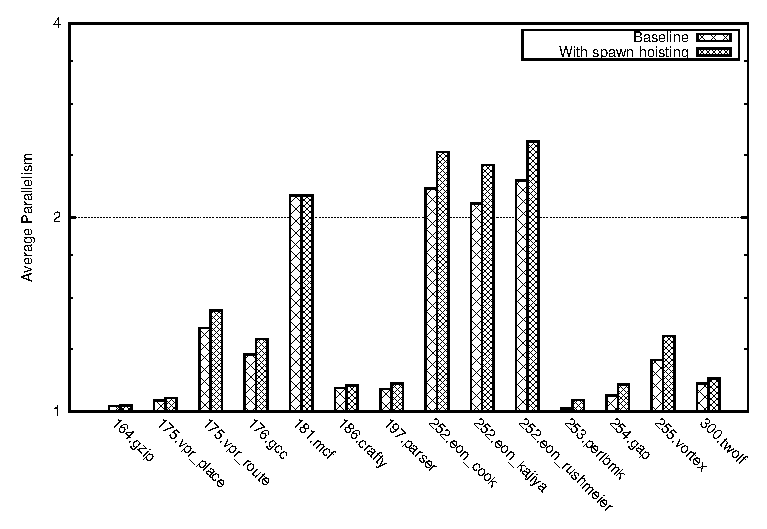
\includegraphics[width=3in]{spec-hoist}
 \caption{Limits of parallelism with and without hoisting spawns}
 \label{spec-hoist}
\end{figure}

The effects of spawn hoisting are presented in Figure \ref{spec-hoist}, which shows the limits of parallelism with and without the optimisation.
While spawn hoisting is useful in the eon benchmark in particular, for most cases the difference it makes is marginal.
On average it results in a 5.5\% speed-up over the baseline.
Nevertheless, this appears to be a relatively straightforward optimisation with few overheads incurred, and as such there is no reason for it to be excluded when performing thread extraction.

\subsection{Other benchmarks}

\begin{figure}
 \centering
 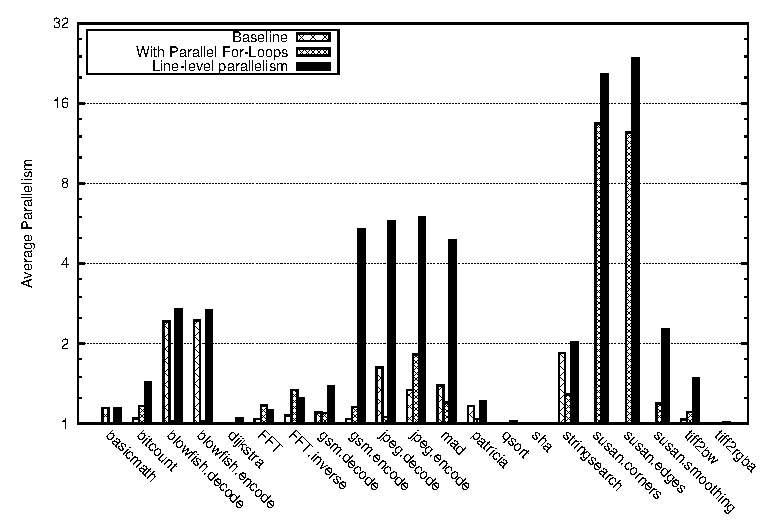
\includegraphics[width=3in]{mb-gran}
 \caption{Limits of parallelism of different granularities in miBench benchmarks}
 \label{mb-gran}
\end{figure}

In addition to the SPEC integer suite, we have also run the same analysis on some of the miBench \cite{guthaus01mibench} suite of application benchmarks for embedded processors, the results of which are presented in Figure \ref{mb-gran}.
The average parallelism of these applications are generally comparable to those of SPEC.
One notable exception, however, is the SUSAN benchmark, which exhibits a much higher degree of parallelism than the rest.
This program performs image smoothing, corner detection and edge detection on an image, and is data-parallel---the same computation is performed on each pixel in the image and the results for each pixel are independent of each other.
As our results show, this parallelism is mainly loop-level.

\subsection{Validation}

\begin{figure}
 \centering
 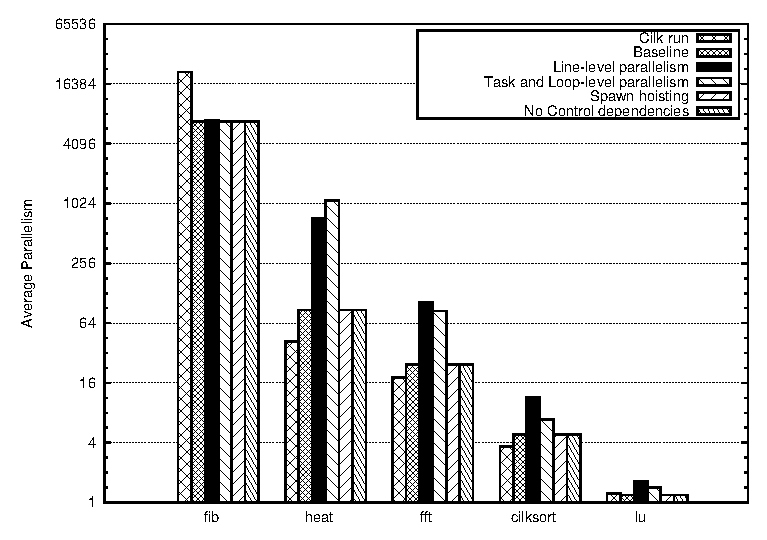
\includegraphics[width=3in]{cilk}
 \caption{Limits of parallelism in Cilk programs}
 \label{cilk}
\end{figure}

To ensure that our model can discover all of the parallelism expressible using popular thread libraries, we used a number of example Cilk programs packaged with the version 5.4.6 release of Cilk, the results of which are displayed in Figure \ref{cilk}.
The leftmost columns show the span measurement that Cilk performs when running these programs on a four-core Linux machine, which is the maximum speed-up given a sufficient number of processors.
The others show the results of running Embla over the same programs with the Cilk keywords removed, i.e.\ their sequential versions.
The span measured by Cilk is in general comparable to the limits computed by Embla using the baseline model, which is the most similar model---this validates that Embla is able to find most if not all of the parallelism expressible in Cilk.
In fact, our results show there is still room for improvement if we allow loop-level parallelism, which Cilk currently does not support\footnote{We note however that Cilk++, a commercialised version, does support parallel for-loops.}.

It can be easily seen by looking at the scale of the y-axis that potential parallelism for most of these programs is much higher than can be found in the SPEC or miBench benchmarks.
This suggests that while a small number of programs have lots of inherent task-level parallelism, general-purpose programs that are not `embarrassingly parallel' have little and cannot be transformed into highly concurrent programs simply by spawning existing function calls and loops.

\subsection{Discussion}

On top of calculating limits of parallelism, Embla also allows us to focus on the critical path and examine the bottlenecks that prevent greater parallelism from being realised.
Using Embla, we have examined several programs in more detail, and we now present some of the reasons why they exhibit such low levels of parallelism, and suggest what can be done to increase their potential.

\subsubsection{186.crafty}

Crafty is a chess-playing program that uses a Minimax-like algorithm to find the best move through searching a game tree.
In theory game tree searching is an easily parallelisable activity, as demonstrated by the success of multi-threaded chess-playing programs \cite{Dailey01usingcilk}.
However, Embla does not find plenty of parallelism in Crafty for a number of reasons.
Firstly, Crafty uses one global chessboard, which is updated when a move is considered and then reverted afterwards, creating a chain of data dependencies that linearise the search.
Furthermore, various pruning techniques used mean that later searches are influenced by the results of earlier ones.
This shows that algorithmic changes are required before such a program can be parallelised.

\subsubsection{164.gzip}

Gzip is a file compression program.
It works by traversing the input file sequentially, looking for recurrences of substrings that have been seen before.
As such it is easy to see that the program cannot process the later parts of the file before the earlier parts have been processed---this results in little task-level parallelism.

\subsubsection{Input/output}

We find that input/output forms a large part of several benchmarks.
In dijkstra, for example, a tenth of the program's sequential execution time is taken up by calls to \texttt{scanf}.
In FFT (miBench), printing the results takes up around 80\% of processing time.
If we assume that input/output is unparallelisable, Amdahl's law would mean that the maximum speed-up, even if we were able to parallelise the rest of the program perfectly, would still be low.
This suggests that for some of the benchmarks examined, a parallel implementation of input/output would be very useful.

\subsubsection{Getting more parallelism from loops}

\begin{figure}
  \centering
  \begin{subfloat}
    \begin{minipage}{3in}
      \begin{verbatim}
for (j = n = 0, seed = rand();
     j < iterations;
     j++, seed += 13) {
  int r = pBitCntFunc[i](seed);
  n += r;
}
      \end{verbatim}
    \end{minipage}%
    \label{orig}
    \caption{Original program}
  \end{subfloat}%
\\
  \begin{subfloat}
    \label{dnc-trans}
    \begin{minipage}{3in}
      \begin{verbatim}
int dc_bitcnts(int start, int n_itrs, int i) {
  if (n_itrs <= 0) return 0;
  if (n_itrs == 1) return pBitCntFunc[i](start);
  else {
    int x,y;
    int half_itrs = n_itrs / 2;
    x = dc_bitcnts(start, half_itrs, i);
    y = dc_bitcnts(start+(half_itrs*13),
          n_itrs - half_itrs, i);
    return x+y;
  }
}

n = dc_bitcnts(seed, iterations, i);
      \end{verbatim}
    \end{minipage}%
    \caption{Transformed program}
  \end{subfloat}%
  \caption{Tranformation of a loop in the bitcount program using divide and conquer.}
  \label{dnc}
\end{figure}

Despite the relatively low figures of parallelism, we have found some simple ways of discovering greater parallelism by small program modifications, one of which we present here.
Figure \ref{dnc} shows the manual transformation applied to a (slightly adapted) loop in the bitcount benchmark.
In the original program, calls to \texttt{pBitCntFunc[i]} are pure and can be run in parallel with each other.
However, there is a dependency between increments of the induction variables, \texttt{j} and \texttt{seed}, and between additions to the accumulator \texttt{n}, producing two long chains of data dependencies.
However, by recognising that \texttt{n} is a reduction variable we can transform the loop into recursive calls using a divde-and-conquer strategy.
The lengths of the dependency chains on the induction and reduction variables become logarithmic on the number of iterations instead of linear, resulting in a tenfold speed-up over the original program, despite the overheads of extra function calls.
This shows that there are simple transformations that increase potential parallelism significantly.

